\documentclass{article}
\usepackage[T1]{fontenc}
\usepackage[utf8]{inputenc}
\usepackage{lmodern}
\usepackage{amsmath}
\usepackage{sansmath}
\AtBeginDocument{\sansmath}
\renewcommand{\familydefault}{\sfdefault}
\usepackage[paperwidth=19cm,paperheight=14cm,margin=0.4cm]{geometry}
\usepackage{graphicx}
\usepackage{tikz}
\usetikzlibrary{positioning,fit,calc,arrows.meta,backgrounds,decorations.pathreplacing}
\pagestyle{empty}
\setlength{\parindent}{0pt}
\graphicspath{{img/}}

\definecolor{ink}{HTML}{0A0A0A}
\definecolor{muted}{HTML}{6A6A69}
\definecolor{line}{HTML}{BDBDBA}
\definecolor{red}{HTML}{E03A3A}
\definecolor{blue}{HTML}{2E6FE0}
\definecolor{yellow}{HTML}{D9A11A}
\definecolor{green}{HTML}{23A06A}
\definecolor{model}{HTML}{8C8C8A}

\tikzset{
  every picture/.style={font=\sffamily\small, line cap=round, line join=round},
  flecha/.style={-{Stealth[length=2.3mm,width=1.7mm]}, line width=0.7pt, draw=ink},
  grupo/.style={draw=#1, dash pattern=on 3pt off 2pt, line width=0.8pt, rounded corners=2pt, inner sep=6pt},
  titulo/.style={font=\sffamily\small\bfseries, text=#1, anchor=south west, inner sep=1pt},
  foto/.style={inner sep=0pt, outer sep=0pt, draw=ink, line width=0.5pt},
  caja/.style={draw=ink, line width=0.5pt, fill=#1, text=white, font=\sffamily\scriptsize\bfseries,
    text width=3.75cm, minimum height=0.46cm, align=center, inner sep=1.5pt},
  nota/.style={font=\sffamily\scriptsize, text=muted, align=center, inner sep=1pt},
  etapa/.style={font=\sffamily\footnotesize\bfseries, text=ink, align=center, inner sep=1pt},
  paso/.style={draw=ink, line width=0.5pt, fill=#1, text=ink, font=\sffamily\scriptsize, align=center,
    inner sep=3pt, minimum height=0.95cm, text width=2.35cm},
  paso/.default=white,
  grupofondo/.style={draw=#1, line width=0.8pt, fill=#1!6, rounded corners=3pt, inner sep=7pt},
  llave/.style={decorate, decoration={brace, mirror, amplitude=5pt, raise=2pt}, line width=0.7pt, draw=#1},
  llavetexto/.style={font=\sffamily\small\bfseries, text=#1, align=center},
}

\definecolor{pink}{HTML}{E8649F}
\begin{document}
\begin{tikzpicture}

\node[foto] (a) at (0, 1.05) {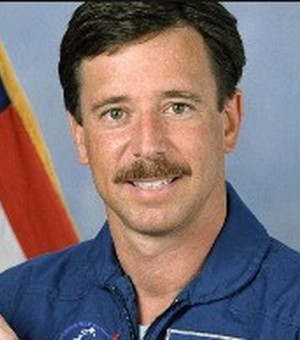
\includegraphics[width=1.45cm]{fi_foto.jpg}};
\node[foto] (b) at (0, -1.25) {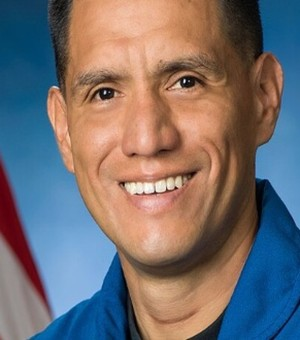
\includegraphics[width=1.45cm]{fi_otra.jpg}};
\node[nota, below=2pt of b] (bl) {otra foto, otra persona\\o la cara guardada};
\node[grupo=muted, fit=(a)(b)(bl)] (g0) {};
\node[titulo=muted] at (g0.north west) {Fotos o cámara};

\node[foto] (pts) at (2.85, -0.1) {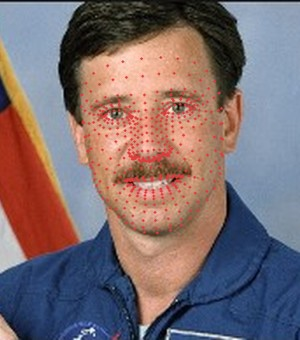
\includegraphics[width=2.05cm]{fi_puntos.jpg}};
\node[etapa, above=4pt of pts] {Puntos};
\node[nota, below=3pt of pts] (ptsl) {468 por cara\\(MediaPipe)};

\node[foto] (mesh) at (5.6, -0.1) {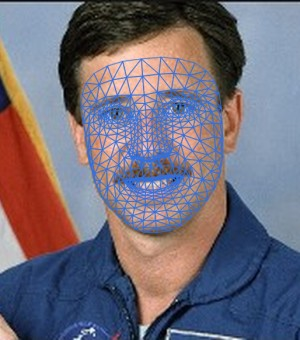
\includegraphics[width=2.05cm]{fi_malla.jpg}};
\node[etapa, above=4pt of mesh] {Malla};
\node[nota, below=3pt of mesh] (meshl) {Delaunay con Fortune,\\una vez, sobre la\\cara promedio};

\node[foto] (r1) at (8.75, 2.05) {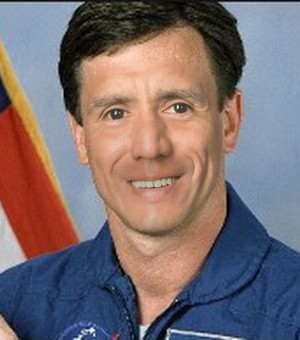
\includegraphics[width=1.3cm]{fi_swap.jpg}};
\node[nota, right=5pt of r1, align=left, text width=3.3cm] (r1l) {\textbf{\color{ink}Cambio de cara}\\warp de la cara donante,\\color de Reinhard y\\mezcla multibanda};
\node[foto] (r2) at (8.75, -0.1) {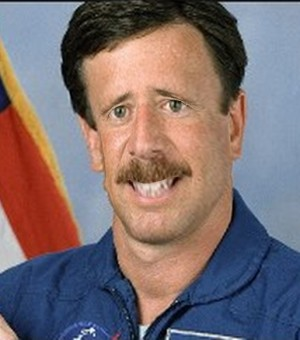
\includegraphics[width=1.3cm]{fi_cari.jpg}};
\node[nota, right=5pt of r2, align=left, text width=3.3cm] (r2l) {\textbf{\color{ink}Caricatura}\\Brennan y escalas locales;\\un anillo fijo deja\\quieto el resto de la foto};
\node[foto] (r3) at (8.75, -2.15) {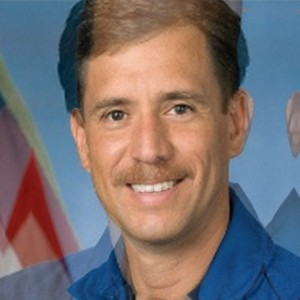
\includegraphics[width=1.3cm]{fi_fusion.jpg}};
\node[nota, right=5pt of r3, align=left, text width=3.3cm] (r3l) {\textbf{\color{ink}Fusión}\\forma intermedia y\\mezcla con pesos $1-t$, $t$;\\$t=0{,}5$ es ``el hijo''};
\node[grupo=pink, fit=(r1)(r1l)(r2)(r2l)(r3)(r3l)] (g3) {};
\node[titulo=pink] at (g3.north west) {Warp afín por triángulo: mapeo inverso y bilineal};

\coordinate (mid) at (0, -0.1);
\draw[flecha] (g0.east |- mid) -- (pts.west);
\draw[flecha] (pts.east) -- (mesh.west);
\coordinate (fan) at ($(mesh.east) + (0.3, 0)$);
\draw[line width=0.7pt, ink] (mesh.east) -- (fan);
\foreach \r in {r1, r2, r3} {
  \draw[flecha, line width=0.5pt] (fan) to[out=0, in=180, looseness=0.9] (\r.west);
}

\coordinate (base) at ($(g3.south) + (0, -0.06)$);
\draw[llave=muted] (pts.west |- base) -- (pts.east |- base)
  node[midway, below=9pt, llavetexto=muted] {Modelo};
\draw[llave=blue] (mesh.west |- base) -- (mesh.east |- base)
  node[midway, below=9pt, llavetexto=blue] {Geometría};
\draw[llave=pink] (g3.west |- base) -- (g3.east |- base)
  node[midway, below=9pt, llavetexto=pink] {Warp, color y mezcla};

\end{tikzpicture}
\end{document}
